
% \documentclass[10pt]{article}
\documentclass[10pt,twocolumn]{article}

% \frenchspacing
% \setlength\parindent{0pt}

\usepackage[english]{babel}
\usepackage[stretch=10, shrink=10]{microtype}
\usepackage[a4paper, total={6.5in, 9in}]{geometry}
\usepackage{graphicx}
\usepackage{caption}
\usepackage{subcaption}
\usepackage{amsmath}
\usepackage{multirow}
\usepackage{xcolor}
\usepackage{hyperref}
\usepackage{float}
\usepackage[linesnumbered,lined,commentsnumbered]{algorithm2e}

% Better vspace in enumerate/itemize
\usepackage{enumitem}
% \setlist{noitemsep,topsep=0pt,parsep=0pt,partopsep=0pt}

\newcommand{\note}[2]{#1${}_{#2}$}
\newcommand{\notesharp}[2]{#1${}_{#2}^{\sharp}$}
\newcommand{\noteflat}[2]{#1${}_{#2}^{\flat}$}

\newcommand{\floor}[1]{\left \lfloor #1 \right \rfloor}
\newcommand{\ceil}[1]{\left \lceil #1 \right \rceil}

% \setlength{\columnsep}{8mm}

\title{\textbf{Real-time monophonic guitar pitch estimation}\\The feasibility of Fourier transform based methods}
\author{Luc de Jonckheere}
% \date{}

\begin{document}
\selectlanguage{english}

\maketitle
%\tableofcontents


\section*{Abstract}
\textcolor{gray}{Short summary.}


\section{Introduction}
Pitch estimation, which is also referred to as f0 estimation, is an important subtask within the field of Automatic Music Transcription (AMT). The goal of pitch estimation is to estimate the pitch or fundamental frequency $f_0$ of a given signal. In the context of AMT, pitch estimation is used to determine what note is played in a given signal.

Real-time pitch estimation is a subproblem where we want to estimate the note associated with the measured pitch while the musician is playing it with minimal latency. This entails we have to use the latest received signal. In contrast to non-real-time methods, we have no knowledge of what may happen ahead of time and signal corresponding to previous notes is irrelevant. This limits the methods we can use to solve this problem.

If pitch estimation can accurately be performed in real-time, it can be used to create a digital (MIDI) instrument from an acoustic instrument. This digital instrument can then be used as an input for audio synthesizers, allowing musicians to produce sounds from a wide variety of instruments. Furthermore, accurate real-time pitch estimation can be used to automatically correct detuned instruments by pitch shifting the original signal to the closest harmonious note.

The Fourier transform is often used to decompose a signal into the frequencies that make up the signal. Predominant frequencies in the signal show up as spectral peaks in the frequency domain. These peaks are important to human perception of melody~\cite{hearing}. %The popularity of the Fourier transform in pitch estimation is likely due to its widespread use in
Other popular methods used for pitch estimation include non-negative matrix factorization, autocorrelation, statistical model based estimation and hidden Markov model based estimation.

Our research focusses on monophonic pitch estimation. Here, we assume that the signal contains at most one note. It is much easier to perform monophonic pitch estimation compared to polyphonic pitch estimation~\cite{monotopoly}, especially when using Fourier transform based methods, as fundamental limits of the Fourier transform inhibit our ability to discern two low pitched notes~\cite{nopoly}. Furthermore, hexaphonic guitar pickups are becoming more widespread, which allows us to view the guitar as six monophonic instruments instead of one six-way polyphonic instrument. Commercial guitar synthesizer solutions from companies with big research departments such as Roland also use these hexaphonic pick-ups, which indicates the infeasibility of accurate and responsive polyphonic pitch estimation of a guitar.

This thesis builds upon a preliminary research project~\cite{ik}. In our research project, we found that Fourier transform based pitch estimation methods might not be well suited for real-time use due to fundamental limitations of the Fourier transform. In this work, we will further research if Fourier transform based methods are viable, as real-time transcription research often relies Fourier transform based methods.

The goal of this thesis is to research the limits of Fourier transform based real-time pitch estimation. To correctly assess the limits, we develop a pitch estimation framework. This framework will focus on extensibility and the ability to perform automated tests. This is important, as much work in this field does not provide its associated source code. This limits the ability to build on other's work and hinders direct comparisons between different methods. Our framework can provide a common ground for the different methods and algorithms to be implemented and compared in. The framework is available at \url{www.github.com/lucmans/digistring}


\section{Related work}
\textcolor{gray}{Other papers. Sample citations~\cite{mono}~\cite{window}~\cite{twotimes}.}


\section{Preliminaries}
\textcolor{gray}{Jargon required to understand this paper.}

\subsection{Audio processing}
\textcolor{gray}{Audio is represented by samples. We get these samples from the OS audio driver. Driver latency.}

\subsection{Fourier transform}
% \textcolor{gray}{Emphasis on discrete FFT (where most papers only mention continuous, which causes misconceptions). Effect of sampling rate (which is often chosen too low) and frame size. Sensitivity for specific frequencies. Quadratic interpolation.}
The Fourier transform is a mathematical transform which transforms a function of time to a complex valued function of frequency and phase. Here, the magnitude represents the amplitude and the argument represents the phase of the corresponding sine wave. The Fourier transform works on continuous functions and assumes an infinite time interval. Concepts such as continuous and infinite cannot be represented by a computer. Consequently, the discrete Fourier transform (DFT) has to be used for Fourier analyses on computers. It can by efficiently implemented used the fast Fourier transform (FFT) algorithm.

The DFT transform a finite sequence of equally spaced samples, which we will refer to as a frame, into an equal number of complex values representing the amplitude and phase, which we refer to as bins. When working with audio, the samples are real valued, and the DFT output is symmetrical. Because of this, we can discard the second half of the output. In the rest of this thesis, we will only consider the first half of the output. Each bin corresponds to a specific frequency. All other frequencies are spread out over other bis, which will be discussed later. Given a frame $F$, the number of samples is the frame is $n_F = |F|$. Using $n_F$ and sample rate $f_{\text{SR}}$, we can calculate the distance between bins:
\[ \Delta f_{bin} = \frac{f_{\text{SR}}}{n_F} \]
This is also referred to as the frequency resolution. Closely related to the frequency resolution is the frame length, which is calculated as follows:
\[ t_F = \frac{n_F}{f_{\text{SR}}} \]
Given a bin number $i \in [0, \floor{\frac{n_F}{2}}]$, the frequency of a bin can be calculated as:
\[ f_{bin} = \Delta f_{bin} * i \]
The 0 Hz bin corresponds to the so called DC offset. This is the average amplitude of the signal. The frequency of the last bin is also called the Nyquist frequency, which is the highest frequency which can be sampled without aliasing. The Nyquist frequency is equal to half the sample rate.

The DFT assumes the frame to be periodic. In other words, the frame is regarded as infinitely repeating. For instance, say we are performing the DFT on a sine wave. If our frame contains 3.33 periods, it will appear as seen in Figure~\ref{fig:framealias} to our DFT. Because of this, some other frequencies also fit the wave in the frame, which is called spectral leakage. Spectral leakage can be controlled used window functions.
\begin{figure}[H]
    \centering
    % 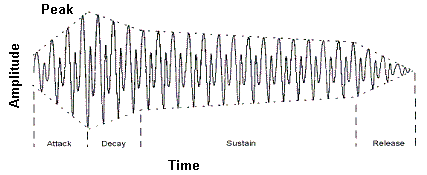
\includegraphics[width=\linewidth]{fig/envelope.png}
    \caption{Aliasing that occurs when performing the discrete Fourier transform}
    \label{fig:framealias}
\end{figure}

% The other frequencies in the input get spread out over all bins, depending on the window function used.

\subsection{Real-time}
Real-time is a difficult concept, as it has many definitions. Here are a few examples of relevant definitions:
\begin{enumerate}
    \item Being synced with actual clock time (or wall time). This is for instance relevant when playing media such as audio and video. When such media is played at an incorrect speed, it could be considered distorted. The hardware which keeps track of the clock time is called a real-time clock.
    \item A system must response within a specified time constraint, which is called the real-time constraint or deadline. This constraint is usually a relatively short time. This definition comes from real-time computing and is relevant when making car airbags or airplane control systems. Failing to response within the real-time constraint leads to failures of the system. Real-time systems are often classified into hard, firm and soft real-time based on the impact of missing the deadline~\cite{realclass}. Note that system that have to respond seemingly instantaneous, such as graphical user interfaces or instant chatting/calling, are not real-time. There are no hard deadlines which the system has to respond within and the system does not fail if some delay does occur. Only user experience is slightly impacted.
    \item \textcolor{red}{A system that can process data faster than it acquires data.} This is technically not real-time, however, it is often used as such in academic literature. It is important for real-time system to process data faster than it acquires it so it does not start to lag behind, however, this is an implicit deadline. Not having this deadline explicit may lead to non-sensible expectations of the system.
\end{enumerate}
Even though the first definition is very relevant when working with audio, it is not relevant for us. The audio drivers of operating systems handle all timing for us. We simply have to wait for samples to be recorded and made available to our program. We only have to keep the sampling rate in mind when working directly with the samples.

In order to allow guitarists to use their guitar as a MIDI instrument, our system has to respond within a small time frame. On top of that, if the system fails to respond quickly enough, the usefulness of the result degrades, as timing is very important when playing an instrument. These restrictions would classify our system as a soft real-time system. We choose a real-time of constraint of TODO milliseconds. We elaborate on this choice in section~\ref{sec:constraint}.

Other work in real-time pitch estimation often uses the third definition of real-time. This is a problem when using Fourier transform based methods, as many papers choose large frame sizes to get a high resolution in the frequency domain. For instance, in order to discern the two lowest notes on a guitar which are 4.9 Hz apart, we would need a frame length of 204 milliseconds. This is well over our real-time constraint and would be unplayable for any musician. Other papers which do explicitly set a real-time constraint, choose very high constraints between 120 ms up to 250 ms. We have found no papers which choose a sensible real-time constraint.

\subsection{Music theory and notation}
In modern western music, we use the twelve-tone equal temperament (12-TET) music system. This system divides an octave, which is the interval between a pitch and another pitch with double the frequency, into twelve equally spaced semitones on the logarithmic scale. The logarithmic scale is used such that the perceived interval between two adjacent notes is constant~\cite{perception}. Moreover, the ratio between two frequencies in an $n$-semitone interval is $\sqrt[12]{2}^n$ or $2^{\frac{n}{12}}$, invariant to pitch.

Using scientific pitch notation, every note can be uniquely identified by combining the traditional note names \note{A}{} to \note{G}{} (with accidentals such as $\sharp$ and $\flat$) with an octave number (e.g. \noteflat{E}{3}). An octave starts at \note{C}{}, which means the octave number increases between \note{B}{} and \note{C}{}. This counter intuitively implies that \note{A}{3} is higher than \note{C}{3}. Note that in 12-TET, \notesharp{C}{} and \noteflat{D}{} are enharmonically equivalent. %Furthermore, even though technically \notesharp{B}{3} (which is equal to \note{C}{4}) is within the fourth octave, it is denoted to be in the third octave as accidentals do not change the octave number.
The range of a typical guitar in standard tuning is from \note{E}{2} up to \note{E}{6}.

The 12-TET music system only describes the relation between two notes in an interval. In order to play with other musicians in harmony, an arbitrary note has to be tuned to a specific frequency. Per ISO 16, the standard tuning frequency of the \note{A}{4} is 440 Hz within an accuracy of 0.5 Hz~\cite{isoa}.

\subsection{Envelope and transients}
The perceived loudness of a note over time can be described using an ADSR envelope. The ADSR envelope of a played note is the convex hull of the waveform of the signal, see Figure~\ref{fig:adsr} for an example. This convex hull can be divided in four parts: Attack, Decay, Sustain, Release. When a note is strummed on the guitar, a percussive sound is generated which causes a loud and sharp attack along with the note. This percussive sound quickly decays and only the actually fretted note will sustain. Finally, when the note is released, it dies out quickly.
\begin{figure}[H]
    \centering
    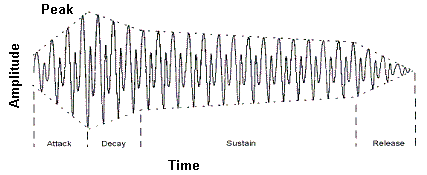
\includegraphics[width=\linewidth]{fig/envelope.png}
    \caption{Example of an ADSR envelope (TODO: Better image)}
    \label{fig:adsr}
\end{figure}

As mentioned before, when strumming a note, a percussive sound is generated. This sound is called a transient and contains a high degree of non-periodic components. Transients appear very chaotically in the frequency domain and thus is often considered as noise. Since a transient is of high amplitude, it overshadows the note that will eventually sustain. Because of this, we cannot use the samples from a transient for pitch estimation. This in turn increases our minimum latency, as we have to wait for samples which do not contain the transient any more.

\subsection{Fundamental frequency, overtones and timbre}
When playing a note on an instrument, many sine waves are generated. The most notable frequency is called the fundamental frequency and determines what note is actually played. Integer multiples of the fundamental frequency can resonate and give rise to harmonic overtones~\cite{overtones}. In practice, these overtones are not exact integer multiples due to non-linear effect.%, however, they are of lower order and can be discarded.
\textcolor{gray}{TODO?: Overtone dissonance.}

Furthermore, many other frequencies are generated along with the fundamental and its overtones. The instrument specific pattern of these frequencies, along with its envelope, is called the timbre of the instrument~\cite{timbre}. The timbre is what separates the sound of the same note played on two different instruments~\cite{perception}. Generally, the amplitude of the timbre frequencies is low compared to the fundamental frequency and can be disregarded as noise in the frequency domain.


\section{Thesis content}
\textcolor{gray}{Actual research etc. Summary what was done in the research project that we build on. Notes on future work of research project.}

\subsection{Real-time constraint}  \label{sec:constraint}
\textcolor{gray}{Start with the factors coming into play when choosing the real-time constraint for our system (latency, played notes per second etc). Note on measured latency in Appendix~\ref{sec:ax100}. Empirically found bounds on latency using our latency program}

\subsection{Software amplification}
\textcolor{gray}{(Software representation of samples and FFT). The FFT works on floating point numbers but most audio interfaces give up to 24 bit integers...}
\textcolor{gray}{We found empirically that when amplifying the input signal in software, peaks in the frequency domain are much easier to detect. However, it has to be done carefully to prevent distortion artifacts.}


\section{Implementation}
\textcolor{gray}{Details about the program I've written. Usage instructions, code choices, code structure, screenshots, expandability}


\section{Experiments}  \label{sec:exp}
\textcolor{gray}{Note that the parameters were empirically optimized with informal experiments. Datasets. Actual experiments.}


\section{Conclusions}
\textcolor{gray}{What we did in this thesis. Reflection on the performance of the system. Final reference to the source code.}


\section{Future work}  \label{sec:future}
\textcolor{gray}{What could still be improved/further researched.}



\appendix
\section{Measuring the latency of the AXON AX 100 mkII}  \label{sec:ax100}
\textcolor{gray}{Lekker meten en weten.}

\section{Effect of different window functions}
\textcolor{gray}{Plots met effect van verschillende window functions.}


\addcontentsline{toc}{chapter}{Bibliography}
\bibliographystyle{plain}
\bibliography{thesis}

\end{document}
 